% Journal Paper on Commutation control of an MRI-powered and imaged Actuator


\documentclass[letterpaper, 10 pt, conference]{ieeeconf}
\IEEEoverridecommandlockouts
\usepackage{calc}
\usepackage{url}
\usepackage[hidelinks]{hyperref}
\usepackage{graphicx}
\usepackage[cmex10]{amsmath}
\usepackage{amssymb}
\usepackage{rotating}

\usepackage{nicefrac}
\usepackage{cite}
\usepackage[caption=false,font=footnotesize]{subfig}
\usepackage[usenames, dvipsnames]{color}
\usepackage{colortbl}
\usepackage{overpic}
\graphicspath{{./pictures/pdf/},{./pictures/ps/},{./pictures/png/},{./pictures/jpg/}}
\usepackage{breqn} %for breaking equations automatically
\usepackage[ruled]{algorithm}
\usepackage{algpseudocode}
\usepackage{multirow}
\usepackage{soul}
\usepackage{bm}   % boldface math type


\newcommand{\topic}[1]{\textcolor{ForestGreen}{\footnotesize \textsf{#1}}}
\newcommand{\todo}[1]{\textcolor{red}{\footnotesize \textsf{#1}}}


%% ABBREVIATIONS
\newcommand{\qstart}{q_{\text{start}}}
\newcommand{\qgoal}{q_{\text{goal}}}
\newcommand{\pstart}{p_{\text{start}}}
\newcommand{\pgoal}{p_{\text{goal}}}
\newcommand{\xstart}{x_{\text{start}}}
\newcommand{\xgoal}{x_{\text{goal}}}
\newcommand{\ystart}{y_{\text{start}}}
\newcommand{\ygoal}{y_{\text{goal}}}
\newcommand{\gammastart}{\gamma_{\text{start}}}
\newcommand{\gammagoal}{\gamma_{\text{goal}}}
\providecommand{\proc}[1]{\textsc{#1}}




\providecommand{\abs}[1]{\left\lvert#1\right\rvert}
\providecommand{\norm}[1]{\left\lVert#1\right\rVert}
\providecommand{\normn}[2]{\left\lVert#1\right\rVert_#2}
\providecommand{\dualnorm}[1]{\norm{#1}_\ast}
\providecommand{\dualnormn}[2]{\norm{#1}_{#2\ast}}
\providecommand{\set}[1]{\lbrace\,#1\,\rbrace}
\providecommand{\cset}[2]{\lbrace\,{#1}\nobreak\mid\nobreak{#2}\,\rbrace}
\providecommand{\lscal}{<}
\providecommand{\gscal}{>}
\providecommand{\lvect}{\prec}
\providecommand{\gvect}{\succ}
\providecommand{\leqscal}{\leq}
\providecommand{\geqscal}{\geq}
\providecommand{\leqvect}{\preceq}
\providecommand{\geqvect}{\succeq}
\providecommand{\onevect}{\mathbf{1}}
\providecommand{\zerovect}{\mathbf{0}}
\providecommand{\field}[1]{\mathbb{#1}}
\providecommand{\C}{\field{C}}
\providecommand{\R}{\field{R}}
\newcommand{\Cspace}{\mathcal{Q}}
\newcommand{\Uspace}{\mathcal{U}}
\providecommand{\Fspace}{\Cspace_\text{free}}
\providecommand{\Hcal}{$\mathcal{H}$}
\providecommand{\Vcal}{$\mathcal{V}$}
\DeclareMathOperator{\conv}{conv}
\DeclareMathOperator{\cone}{cone}
\DeclareMathOperator{\homog}{homog}
\DeclareMathOperator{\domain}{dom}
\DeclareMathOperator{\range}{range}
\DeclareMathOperator{\sign}{sgn}
\DeclareMathOperator{\sgn}{sgn}
\providecommand{\polar}{\triangle}
\providecommand{\ainner}{\underline{a}}
\providecommand{\aouter}{\overline{a}}
\providecommand{\binner}{\underline{b}}
\providecommand{\bouter}{\overline{b}}
\newcommand{\D}{\nobreakdash-\textsc{d}}
%\newcommand{\Fspace}{\mathcal{F}}
\providecommand{\Fspace}{\Cspace_\text{free}}
\providecommand{\free}{\text{\{}\mathsf{free}\text{\}}}
\providecommand{\iff}{\Leftrightarrow}
\providecommand{\subinner}[1]{#1_{\text{inner}}}
\providecommand{\subouter}[1]{#1_{\text{outer}}}
\providecommand{\Ppoly}{\mathcal{X}}
\providecommand{\Pproj}{\mathcal{Y}}
\providecommand{\Pinner}{\subinner{\Pproj}}
\providecommand{\Pouter}{\subouter{\Pproj}}
\DeclareMathOperator{\argmax}{arg\,max}
\providecommand{\Aineq}{B}
\providecommand{\Aeq}{A}
\providecommand{\bineq}{u}
\providecommand{\beq}{t}
\DeclareMathOperator{\area}{area}
\newcommand{\contact}[1]{\Cspace_{#1}}
\newcommand{\feasible}[1]{\Fspace_{#1}}
\newcommand{\dd}{\; \mathrm{d}}
\newcommand{\figwid}{0.22\columnwidth}

\DeclareMathOperator{\atan2}{atan2}


\newtheorem{theorem}{Theorem}
\newtheorem{definition}[theorem]{Definition}
\newtheorem{lemma}[theorem]{Lemma}
\begin{document}


%%%%%%%%%%%%%% For debugging purposes, I like to display the TOC
%    \tableofcontents
%    \setcounter{tocdepth}{4}
%    \newpage
%%%%%% END TOC %%%%%%%%%%%%%%%%%%%%%%%%%%%%%%%%%%%%%%%

\title{\LARGE \bf 
Commutation Control of an MRI-Powered and Imaged Actuator
}
\author{ Ouajdi Felfoul, Alina Eqtami, Aaron Becker, and Pierre E.\ Dupont%, 
\thanks{{O.~Felfoul, A. Eqtami, A.~Becker, and P.~E.~Dupont are with the Department of Cardiovascular Surgery,  Boston Children's Hospital and Harvard Medical School, Boston, MA, 02115 USA {\tt\small first name.lastname@childrens.harvard.edu}.
}
} %\end thanks
} % end author block
\maketitle

\begin{abstract}
Actuators that are powered, imaged, and controlled by Magnetic Resonance (MR) scanners offer the potential of inexpensively providing wireless control of MR-guided robots. Similar to traditional electric motors, the MR scanner acts as the stator and generates propulsive torques on an actuator rotor containing one or more ferrous particles. 
\end{abstract}
\todo{\section{tasks}}
\todo{
\begin{enumerate}
\item Debug the sequence that avoids the two-actuation cycle delay in applying rotor angle. 
\item Estimator tasks (most of these are to generate text for paper as well as to justify approach):
\begin{enumerate}
\item
(i) Write out an explanation of what type of estimator will work best for our nonlinear system (Extended Kalman filter, particle filter, etc.) 
        (ii) Explain any linearization / operating point that needs to be used.
        (iii) Write down general equations for selected estimator and then tailor them to our problem.
(iv) Account for measurement delay between projections.
(iv) Write out entire controller as generic algorithm code (as computer scientists do)
\end{enumerate}
\item Once we are convinced that estimator and controller are correct (by performing tasks above), collect data comparing open- and closed-loop performance of rotor. Important data will include maximum torque produced (stall torque), rotor slip versus no slip, angle between gradient and rotor versus time, effect of actuation duration on stall torque and transient performance, demonstration of position control by step response.
\item Alina � could you derive some sort of stability / error bound that we could validate experimentally? If so, what would the validation experiment entail?
\end{enumerate}
}

%%%%%%%%%%%%%%%
\section{Introduction}\label{sec:Intro}
%
 %function and implementation function
 
This project addresses the need for ultra-minimally invasive robots to perform diagnostic and therapeutic tasks deep inside the body while simultaneously addressing the need for integrated real-time imaging. In contrast, most existing approaches employ large robots and consequently require relatively large incisions.  In consequence, substantial healthy tissue can be damages en route to the diseased tissue.  Because of this collateral damage, treatment is often delayed or alternative less-effective techniques are employed.  For example, in brain surgery, it is often necessary to sacrifice functioning brain tissue to reach an underlying tumor.  In  heart disease, less-effective catheterization procedures may be performed to avoid the risks and trauma of open-heart surgery. \todo{ref?}
 
 At the millimeter and sub millimeter scale, groups of MRI-powered swimming robots could perform targeted therapies inside fluid-filled regions of the body, such as the ventricular system of the brain. \todo{figure from NRI?} Because the ventricles provide access to a substantial portion of the brain, the proposed millirobots, injected into the spine and steered to the brain, could significantly reduce the morbidity of current procedures whiles also enabling a broad range of new procedures.  These millirobots could be capable of performing localized therapies such as drug and cell delivery for the treatment of cancer, epilepsy and other diseases.  They could also be capable of forming sensor networks to monitor such quantities as pressure.  As delivery vehicles(of drugs, for example), they would be superior to systemic delivery since they would enable high concentrations to be delivered to very specific locations while bypassing the blood-brain barrier and without exposing the rest of the body.
 
 
 
 
 Math about swimmer bouyancy
 
 Math about dipoles in a very strong magnetic field \cite{thomaszewski2008magnets}
 
 Simulation of many dipoles in a strong magnetic field
 -- 4 dipoles in field, start at random positions, see what shapes are formed.  Do experiment 1000s of times and get shape formation probabilities.
We derive inspiration from simulations by Alink et al.~on self-assembly of 3 to 4 permanent magnets\cite{alink2011simulating}, and simulations of aggregation with nanoparticles in \cite{vartholomeos2010simulation}.
 
 Experiments -- place 2-5 magnets in water,  record ending configurations.  Show this matches simulation (?)
 
 Controlled buoyancy experiments -- show we can make configurations that are unlikely by chance
 
 Show we can make a desired configuration
 
 Steer the assembly around.
 
 
 \subsection{Why MRI?}

 

 Our paper is organized as follows.  After a discussion of related work in Section \ref{sec:RelatedWork}, we describe our model and control law in Section \ref{sec:designAndControl}.  Section \ref{sec:analysis} examines how to optimize system design.   We report the results of our experiments in Section \ref{sec:experiment}, and end with concluding remarks in Section \ref{sec:conclusion}.



%%%%%%%%%%%%%%%
%%%%%%%%%%%%%%%
\section{Multi-Rotor Control}\label{sec:controlLaw}

A ferrous particle in the strong static field of an MRI becomes magnetized, and its magnetization magnitude asymptotically approaches the saturation magnetization $\mathbf{M}_s$ per unit volume of the material.  The MRI gradient coils  produce a magnetic field  $\mathbf{B}_g(t)$. This field exerts 
 on the ferrous particle the force 
\begin{equation}
\mathbf{F}(t) = v\left( \mathbf{M}_s
\cdot \nabla \right) \mathbf{B}_g(t). \label{eq:forceOnDipole}
\end{equation}
Here $v$ is the magnetic volume of the material.  The magnetic field $\mathbf{B}_g(t)$ is designed to produce three independent gradients:
\begin{equation}
\left[ F_x,F_y, F_z \right]^\intercal\!\!(t)= v M_{sz}\left[ 
   \frac{ \partial B_{gz}}{\partial x}, 
   \frac{ \partial B_{gz}}{\partial y},
   \frac{ \partial B_{gz}}{\partial z} 
   \right]^\intercal\!\!\!\!(t)
\label{eq:applicableForces}
\end{equation}
Here it has been reasonably assumed that $M_{sz} \gg M_{sx}, M_{sy}$.
These gradients apply three independent forces on any ferromagnetic spheres inside the MRI.  
 \begin{figure}
 \centering
% \vspace{-1em}
\begin{overpic}[width = 0.85\columnwidth]{Schematic2.pdf}\end{overpic}
 \vspace{-1em}
\caption{
\label{fig:Schematic}
MRI-powered, single-DOF rotor with gear for power transmission.
}
\vspace{-1.5em}
\end{figure}
This paper investigates rotors that constrain the $i$th ferromagnetic sphere to rotate about an axis $\mathbf{a}_i$ with a moment arm of length  $r_i$, as shown in Fig.~\ref{fig:Schematic}.  The rotor's configuration is fully described  by its angular position and velocity $[\theta_i, \dot{\theta}_i]^\intercal$. The configuration space of all $n$ rotors is $\R^{2\times n}$,  and the dynamic equations are

\begin{equation}
J_i\ddot{\theta}_i(t) = -b_i\dot{\theta}_i(t) -\tau_{f_i}-\tau_{\ell_i} + r_i \mathbf{F}\cdot \mathbf{p}_i(t)
\label{eq:rotorDynamics}
\end{equation}
Here $J_i$ is the moment of inertia, $b_i$ the coefficient of viscous friction,  $\tau_{f_i}$ the summation of all non-viscous friction terms seen by the input,  and $\tau_{\ell_i}$ the load torque. The rotor torque is the magnetic force projected  to a vector tangent to the ferrous sphere's positive direction of motion, $r_i \mathbf{F}\cdot \mathbf{p}_i(t)$
Actuator torque is maximized when $\mathbf{F}(t) = g_{M}V M_{sz}\sgn(\mathbf{p}_i(t)) $, where  $g_{M}$ is the maximum gradient.

There are two standard actuator control tasks: position and velocity control. 
%Given $q(0)\in \R^{2\times n}$, and $\bm{\theta}_{\textrm{goal}}\in\R^n$ the position control problem is to find inputs $\mathbf{F}(t)$ such that for any $q(0)$ and $q_{\textrm{goal}}$, 
The position control problem is to find inputs $\mathbf{F}(t)$ such that for any $\bm{\theta}(0)$ and $\bm{\theta}_{\textrm{goal}}$, 
\begin{equation}\lim_{t \to \infty}\sum_{i=1}^n \norm{\begin{bmatrix}\theta_i(t)\\ \dot{\theta}_i(t)\end{bmatrix}-\begin{bmatrix}\theta_{\textrm{goal},i}\\ 0 \end{bmatrix} }_2 = 0.
\end{equation}
This section starts with the simpler velocity control problem
\begin{equation}
\lim_{t \to \infty}\sum_{i=1}^n \norm{ \dot{\theta}_i(t)- \omega_i }_2 = 0,
\end{equation}
where $\omega_i \in \R$ is the desired angular velocity of each rotor. After solving the velocity control problem in Sec. \ref{subsec:ControlLyapunov},   Section \ref{subsec:PositionControl} uses an outer control loop to stabilize position.




\subsection{Open-Loop Multi-Actuator Control}
Before considering closed-loop control, it is worthwhile to determine what can be achieved in open-loop and to examine related performance limitations.  In this context, one method to independently control multiple rotors uses the magnetic field gradients to make the rotors revolve around \emph{orthogonal} axes. For notational simplicity, assume the rotors rotate about the world $x,y,z$ axes.
With $n\le3$ orthogonal rotors,  open-loop control signals can rotate some rotors at constant velocities, and move the remaining rotors to steady-state positions.  For instance, the control law
\begin{equation}
\nabla  \mathbf{B}_g(t) = g_{M} \left[  \cos(t), \sin(t), 0  \right]^\intercal
\end{equation}
rotates the $z$-axis rotor in the positive direction at 1 rad/s  and places the $x$ and $y$ rotors in steady-state positions.

To simultaneously rotate up to three orthogonal rotors, the gradient can be rotated at angular frequency $\omega$ around the vector $\bm{\phi} = \dfrac{[\phi_x,\phi_y,\phi_z]^\intercal}{\sqrt{\phi_x^2+\phi_y^2+\phi_z^2}}$, where $\phi_i \in \{-1,0,1\}$ is the desired rotation of the $i$th axis. This gives the control law
\begin{align}
\label{eq:OpenLoopControlRotors3}
\nabla  \mathbf{B}_g(t) &= g_{M} R_{\bm{\phi},\omega t} \cdot \bm{\phi}_{\perp}.
\end{align}
Here $\bm{\phi}_{\perp}$ is a vector perpendicular to $\bm{\phi}$ and $R_{\bm{\phi},\omega t}$ is the rotation matrix that rotates the angle $\omega t$ about the axis $\bm{\phi}$.  Control law  \eqref{eq:OpenLoopControlRotors3} with three orthogonal rotors has 27 possible outputs.  Figure \ref{fig:OpenLoopRotationsArrow} shows three representative control inputs.  The 2D projections show how rotating the magnetic field around different $\bm{\phi}$ vectors rotates one, two, or three rotors simultaneously.

 \begin{figure}
 \centering
 \begin{minipage}{0.4\linewidth}
\begin{overpic}[width = \columnwidth]{OpenLoopRotationsArrow3.pdf}
\put(54,9){$\theta_x$}
\put(67,53){$\theta_y$}
\put(12,85){$\theta_z$}
\end{overpic}
\end{minipage}~~\begin{minipage}{0.58\linewidth}
\begin{overpic}[width=0.3\textwidth]{projForOpenLoopg2}\put(12,85){$\theta_x$}\end{overpic}
\begin{overpic}[width=0.3\textwidth]{projForOpenLoopg1}\put(12,85){$\theta_z$}\end{overpic}
\begin{overpic}[width=0.3\textwidth]{projForOpenLoopg3}\put(12,85){$\theta_y$}\end{overpic}\\
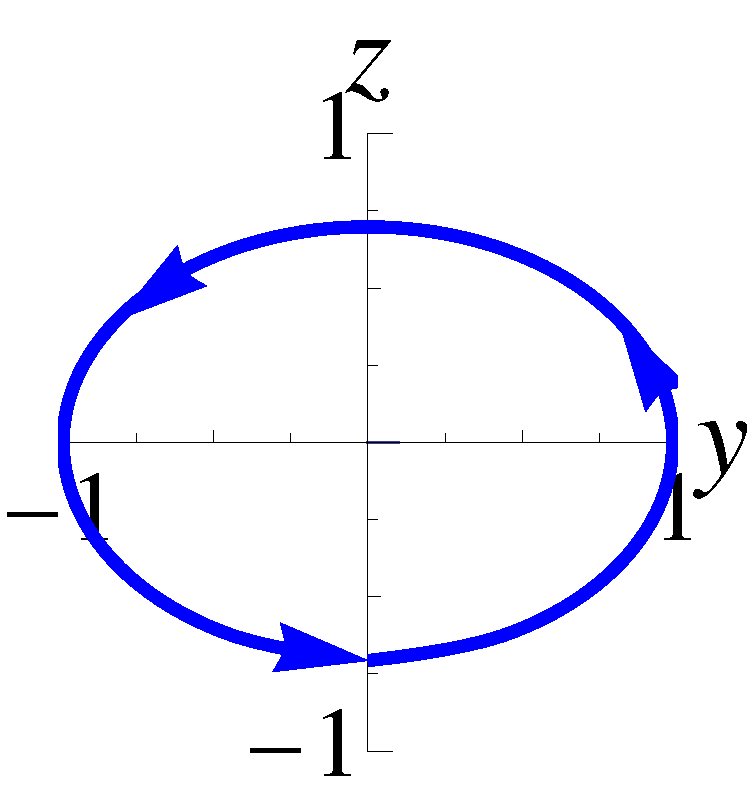
\includegraphics[width=0.3\textwidth]{projForOpenLoopb2}
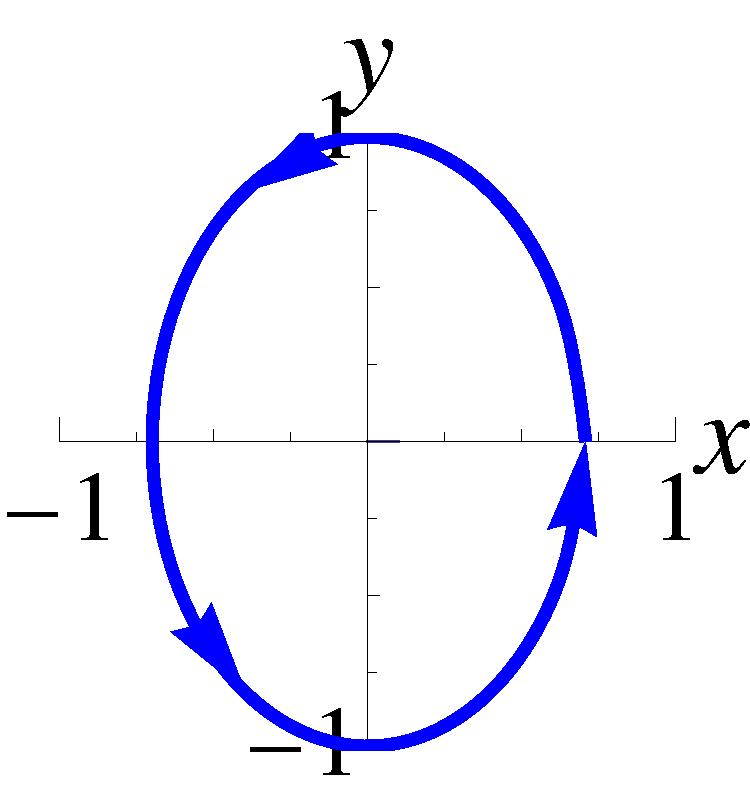
\includegraphics[width=0.3\textwidth]{projForOpenLoopb1}
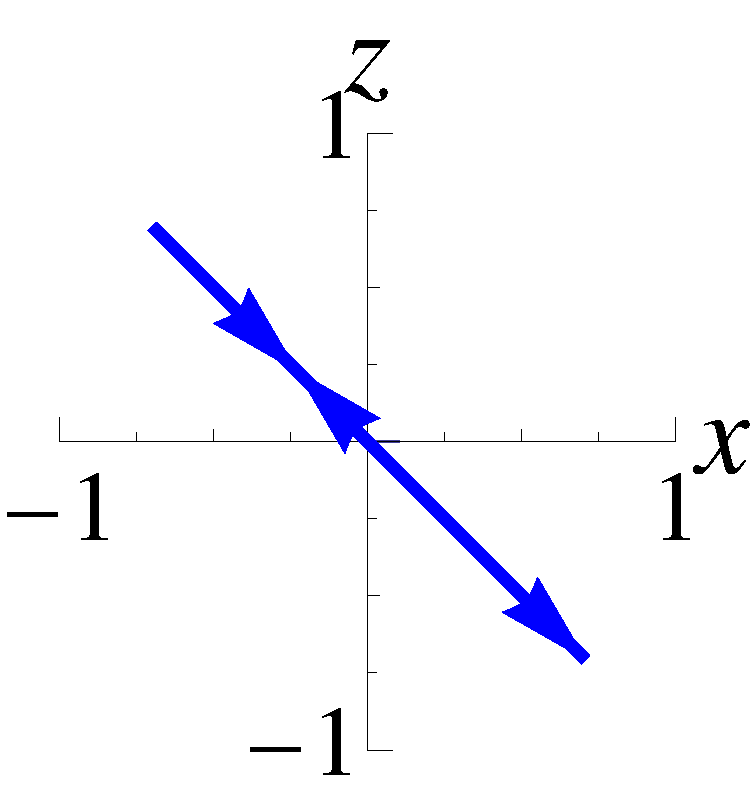
\includegraphics[width=0.3\textwidth]{projForOpenLoopb3}\\
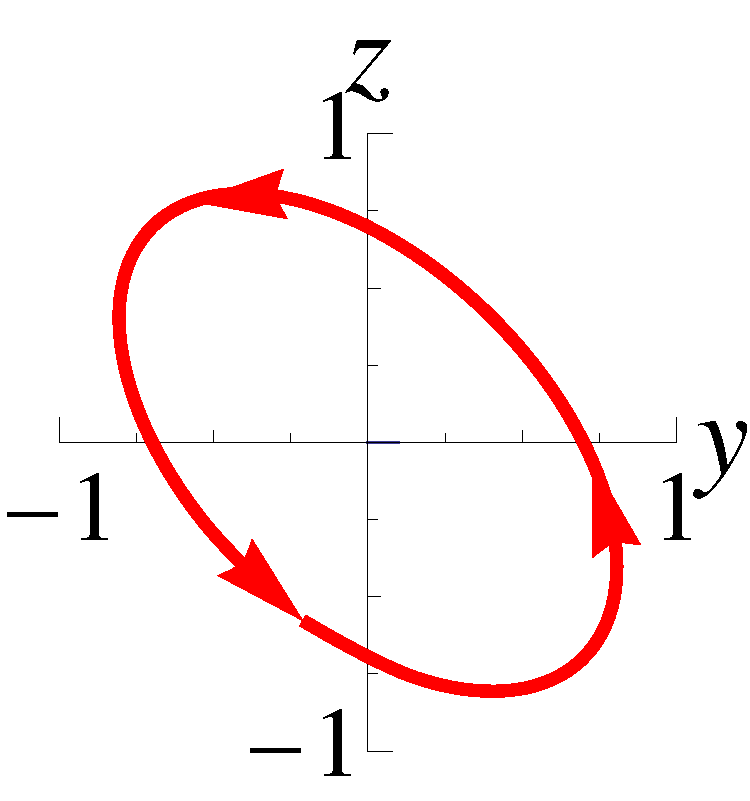
\includegraphics[width=0.3\textwidth]{projForOpenLoopr2}
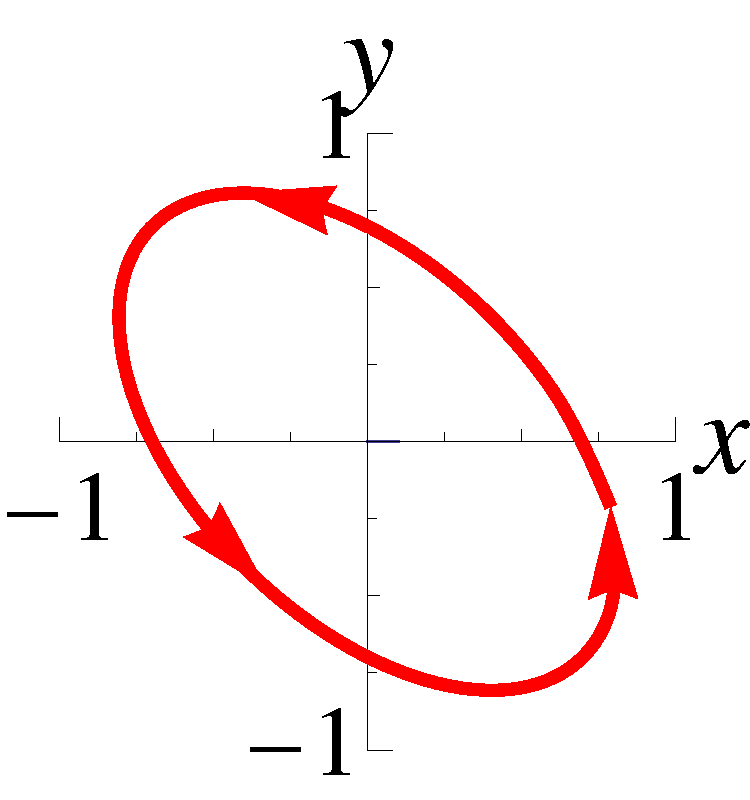
\includegraphics[width=0.3\textwidth]{projForOpenLoopr1}
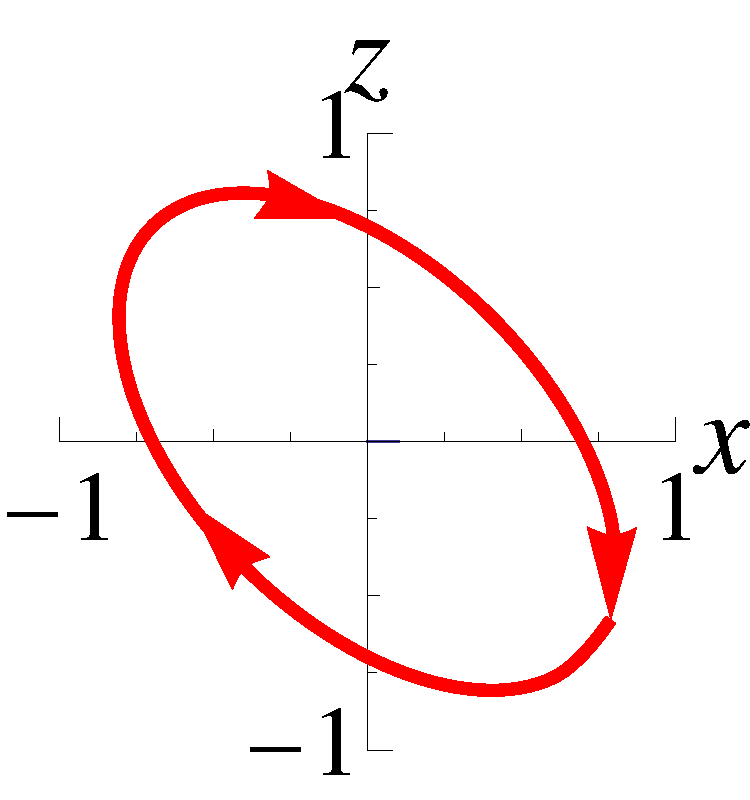
\includegraphics[width=0.3\textwidth]{projForOpenLoopr3}\\
\end{minipage}
\vspace{-1.75em}
\caption{
\label{fig:OpenLoopRotationsArrow}
The open-loop control law  \eqref{eq:OpenLoopControlRotors3} for three orthogonal axes has 27 possible outputs corresponding with: only one rotor spinning (green), two rotors spinning (blue), all three spinning (red), or none spinning. At right are projections onto the three coordinate axes. \href{http://youtu.be/nzym0mABaKY}{See video attachment for experimental verification.}
}\vspace{-2em}
\end{figure}

As demonstrated in these examples, open-loop control has several limitations. For example, rotor velocities are coupled and position control is not possible. In addition, the approach is limited to at most three rotors since their axes must be orthogonal. Furthermore, as shown in the \href{http://youtu.be/nzym0mABaKY}{video attachment}, cyclic slipping of the rotor due to applied load or perturbations is possible. Closed-loop control, described in the following subsection, can eliminate these limitations. 
  \begin{figure*}
\subfloat[positions, 4 rotor  control]{\begin{overpic}[height = 0.206\linewidth]{PositionConverge4state.pdf}\end{overpic}}
\subfloat[control inputs, 4 rotor control]{\begin{overpic}[height = 0.206\linewidth]{PositionConverge4control.pdf}\end{overpic}}
\subfloat[positions, 24 rotor control]{\begin{overpic}[height = 0.206\linewidth]{PositionConverge24state.pdf}\end{overpic}}\vspace{-1.em}\\
\vspace{-1.2em}
\subfloat[positions, 4 rotor  control, no load]{\begin{overpic}[height = 0.206\linewidth]{PositionConverge4stateNoload.pdf}\end{overpic}}
\subfloat[control inputs, 4 rotor control, no load]{\begin{overpic}[height = 0.206\linewidth]{PositionConverge4controlNoload.pdf}\end{overpic}}
\subfloat[positions, 50 rotor control]{\begin{overpic}[height = 0.206\linewidth]{PositionConverge50state.pdf}\end{overpic}}\\
\caption{\label{fig:PositionControlSim}Simulated position control of multiple non-parallel rotors.  }
\vspace{-1.75em}
\end{figure*}
\subsection{Closed-Loop Multi-Actuator Velocity Control }\label{subsec:ControlLyapunov}
   To enable robust, multi-axis control, a closed-loop controller can be designed using a control-Lyapunov function~\cite{Artstein1983}.  The control law selects the three magnetic gradients that decrease the sum of squared velocity error. There are configurations where no combination of velocity gradients will decrease this error, but it is always possible to apply a non-zero gradient without increasing the sum squared error. Any non-zero gradient will move the rotors to a new configuration where the error can be decreased. This technique is inspired by work on controlling many mobile robots with a uniform control signal~\cite{Becker2012k}.
  For ease of analysis, simplified rotor dynamics will be used: 
   \begin{equation}
\ddot{\theta}_i(t) =   \frac{r_i}{J_i} \mathbf{F}(t)\cdot \mathbf{p}_i(t).
\label{eq:rotorDynamicsSimple}
\end{equation}
   In all simulations the full dynamic model \eqref{eq:rotorDynamics} is used.
   
   Given $n$ non-parallel rotors and desired angular velocities $\omega_i$, a suitable Lyapunov function can be defined as the sum squared velocity error:
   \begin{align}
   \label{eq:LyapunovFunction}
   V(\bm{\theta},\dot{\bm{\theta}},t) &= \frac{1}{2} \sum_{i=1}^n \left(  \omega_i - \dot{\theta}_i(t)\right)^2 
      \end{align}
      \begin{align}
   \label{eq:LyapunovFunctionD}
   \dot{V}(\bm{\theta},\dot{\bm{\theta}},t) &=  \sum_{i=1}^n \left( \omega_i - \dot{\theta}_i(t)  \right) \ddot{\theta}_i(t)   \nonumber \\
  &=  \mathbf{F}(t)\cdot \sum_{i=1}^n \left(  \omega_i - \dot{\theta}_i(t) \right) \frac{r_i}{J_i} \mathbf{p}_i(t)
   \end{align}
Note that $V(\bm{\theta},\dot{\bm{\theta}},t)$ is positive definite, zero only at the target velocity, and radially unbounded. The following controller makes $ \dot{V}(\bm{\theta},\dot{\bm{\theta}},t) $ negative semi-definite:
\begin{equation}
\label{eq:velocityControlPolicy}
\mathbf{F}(t) = -g_{M}v_i  M_{sz}\left(  \sum_{i=1}^n \left(  \omega_i - \dot{\theta}_i(t) \right) \frac{r_i}{J_i}  \mathbf{p}_i(t)    \right)
\end{equation}
 For such an $\mathbf{F}(t)$,
   \begin{align*}
  \dot{V}(\bm{\theta},\dot{\bm{\theta}},t) &=  -  g_{M}v_i  M_{sz}\left( \sum_{i=1}^n \left(  \omega_i - \dot{\theta}_i(t) \right) \frac{r_i}{J_i}  \mathbf{p}_i(t) \right)^2.
   \end{align*}
Notice that  $\dot{V}(\bm{\theta},\dot{\bm{\theta}},t)\le0$, but there exists a subspace of $[\bm{\theta}, \dot{\bm{\theta}}]^\intercal$ where $\dot{V}(\bm{\theta},\dot{\bm{\theta}},t)=0$.  Because this derivative is negative semi-definite, the system is stable, but not necessarily asymptotically stable.  To prove asymptotic stability requires proving that the invariant set contains only the rotors moving at the desired angular velocity.  

Control law \eqref{eq:velocityControlPolicy} is modified as follows:
   \begin{align}
\mathbf{f} & = \sgn\!\left(  -\sum_{i=1}^n \left(  \omega_i - \dot{\theta}_i(t) \right) \frac{r_i}{J_i}  \mathbf{p}_i(t)    \right)\nonumber\\
\mathbf{F}(t) &=g_{M}v_i M_{sz}\begin{cases} [1,1,1]^\intercal &\mbox{if } \mathbf{f} = 0 \mbox{ and } \dot{\bm{\theta}} \ne \bm{\omega} \\ 
					       \mathbf{f} & \mbox{else } \end{cases}
					       \label{eq:velocityControlPolicyInv}
   \end{align}
The \emph{signum function} $\sgn(\cdot)$ returns the sign of the argument, or 0 if the argument is zero. 
This ensures that the only invariant state is the target velocity $ \dot{\bm{\theta}} = \bm{\omega}$.  At all other configurations where $\dot{V}(\bm{\theta},\dot{\bm{\theta}},t) = 0$, the control law  \eqref{eq:velocityControlPolicyInv}  generates a nonzero acceleration $\ddot{\theta}_i(t)$ without increasing $V(\bm{\theta},\dot{\bm{\theta}},t)$, and thus some rotors will change velocities.   


\subsection{Closed-Loop Multi-Actuator Position Control}\label{subsec:PositionControl}

 
Position control is possible by implementing a feedback loop around \eqref{eq:velocityControlPolicyInv} with a time-varying $\bm{\omega}(t)$.  Given a desired position vector $\bm{\theta}_{\textrm{goal}}$, a PID controller can be implemented to determine $\bm{\omega}(t)$ based on the position error vector, $\mathbf{e}$:
   \begin{align}
\bm{e}(t) &=\bm{\theta}_{\textrm{goal}} - \bm{\theta}(t)\nonumber \\
\bm{\omega}(t) &= K_{p}  \bm{e}(t) + K_i\int_0^t \bm{e}(\tau) + K_d \frac{d}{dt} \bm{e}(t).
\label{eq:positioncontrol}
   \end{align}
 Note that $\theta_{\textrm{goal}}$ and $\theta_i(t)$ are real numbers and are not wrapped to $[-\pi,\pi]$. The three gain parameters may be set to achieve application-specific requirements.  In simulations, $[K_{p},K_i,K_d]=[10,0,0]$ and $\bm{e}(t)$ is saturated to  $\pm 50$.
 

 

 Control policy  \eqref{eq:positioncontrol} scales to large numbers of rotors.  For example, Fig.~\ref{fig:PositionControlSim} shows simultaneous convergence to prescribed angular positions for 4, 24, and 50 rotors. All show asymptotic convergence, but convergence time increases with the number of rotors. With no load there is asymptotic convergence, but a non-zero load oscillates about $\bm{\theta}_{\textrm{goal}}$ because not all final configurations can be statically held by a constant gradient field.
 The simulated dynamic parameters used  in \eqref{eq:rotorDynamics} are below:
%$r_{sphere} = 6$mm,
% $m_{sphere} = 7.7$g,
%  $r_i  = 18$mm,
% $J_i = 2m_{sphere}  r_i^2$kgm$^2$,
% $b_i =  1\times 10^{-7}$Nms/rad,
% $\tau_{f_i} =  7\times 10^{-5}$Nm.
\setlength{\tabcolsep}{1pt}      
\begin{center}
\begin{tabular}{  r l  @{\hskip .5in}  r l }      
$r_{sphere}$&$= 6$mm 				&  $\tau_{f_i}$&$=  7\times 10^{-5}$Nm  \\
$m_{sphere}$&$= 7.7$g  				&  $b_i $&$=  1\times 10^{-7}$Nms/rad \\
 $r_i  $&$= 18$mm					&   $J_i $&$= 2m_{sphere}  r_i^2$ kgm$^2$\\
\end{tabular}
\end{center}
The load torques $\tau_{\ell_i}$ are set $\pm1\times 10^{-5}$Nm with a random half set negative and the rest positive.  \href{http://www.mathworks.com/matlabcentral/fileexchange/45331}{These {\sc Matlab} simulations are available online}~\cite{Becker2014b}.


%%%%%%%%%%%%%%%
%%%%%%%%%%%%%%%
%%%%%%%%%%%%%%%%%%%%%%%%%%%%%%%%%%%%%%%%%%%%%%%%%%%%%%%%%%%%
\section{Multi-Actuator Design Constraints}
\label{sec:analysis}
%%%%%%%%%%%%%%%%%%%%%%%%%%%%%%%%%%%%%%%%%%%%%%%%%%%%%%%%%%%
The preceding section demonstrated how closed-loop control can independently control multiple rotors.  Given this capability, there are constraints that must be respected when designing an MRI powered and controlled multi-actuator system.  These involve (1) arranging the rotors to minimize interaction forces, (2) MRI imaging-based tracking of each rotor, (3) geometrically arranging the rotor axes to maximize torque, and (4) calculating the stall torque as a function of the number of actuators. Each of these is described below.

%Using multiple rotors simultaneously in the same MR scanner introduces challenges not seen with only one rotor.  This section analyzes the magnetic interaction between the ferrous spheres, interference when imaging, and questions about the optimal placement of the rotors.


\subsection{Actuator Interaction Forces}\label{subsec:minimumseparation}
Any ferrous material placed in the magnetic field of an MR scanner becomes a strong magnetic dipole.  With multiple MR-powered motors, these dipoles exert forces on each other.  Dipole forces overpower MRI gradient forces if rotors are closer than a threshold distance.

The magnetic field at position $\mathbf{r}_2$ generated by a spherical magnet at position $\mathbf{r}_1$ with magnetization  $\mathbf{m}_1$ is  \cite{Schill2003} %\cite{thomaszewski2008magnets}
\begin{align}
\label{eq:dipoleMagField}
 \mathbf{B}_{\mathbf{r}_1}(\mathbf{r_2}) = \frac{\mu_0}{4 \pi}\frac{3 \mathbf{n}_{12}(\mathbf{n}_{12} \cdot \mathbf{m}_1) - \mathbf{m}_1}
 {|\mathbf{r}_2-\mathbf{r}_1|^3},
\end{align}
with  $\mathbf{n}_{12} = (\mathbf{r}_2-\mathbf{r}_1)/|\mathbf{r}_2-\mathbf{r}_1|$. This is the \emph{magnetic field of a dipole}.
 The force applied to a dipole at $\mathbf{r}_1$ with magnetic moment $\mathbf{m}_1$ by another dipole at $\mathbf{r}_2$ with magnetic moment $\mathbf{m}_2$ is approximated by
\begin{align}
\mathbf{F}_{12} \approx \frac{3\mu_0}{4 \pi} \frac{1}{|\mathbf{r}_2 - \mathbf{r}_1 |^4}
\left[5 \mathbf{n}_{12}\Big(\left(\mathbf{m}_1 \cdot \mathbf{n}_{12} \right)   \left(\mathbf{m}_2 \cdot \mathbf{n}_{12} \right) \Big) \right. \nonumber \\
\left.
-  \mathbf{n}_{12} \left(\mathbf{m}_2 \cdot \mathbf{m}_1 \right)
-  \mathbf{m}_{1} \left(\mathbf{m}_2 \cdot \mathbf{n}_{12} \right)  -  \mathbf{m}_{2} \left(\mathbf{m}_1 \cdot \mathbf{n}_{12}\right)   \right].\nonumber
\label{eq:dipoleForce}
\end{align}

 \begin{figure}
 \centering
\begin{overpic}[height = 0.47\columnwidth]{MagneticDipoleField3mmRast}
\tiny
\put(28,29){0}
\put(28,73){0}
\put(89,73){0}
\put(89,29){0}
\put(27,51){-0.1$g_{M}$}
\put(52,17){0.1$g_{M}$}
\put(56,38){$g_{M}$}
\put(64.5,52){-$g_{M}$}
\small
\put(35,-8){$r_{sphere}$ = 3mm}
\end{overpic}
\begin{overpic}[height = 0.47\columnwidth]{MagneticDipoleField6mmRast}
\tiny
\put(20,29){0}
\put(20,79){0}
\put(89,79){0}
\put(89,30){0}
\put(15,70){-0.1$g_{M}$}
\put(25,15){0.1$g_{M}$}
\put(52,38){$g_{M}$}
\put(68.5,55){-$g_{M}$}
\small
\put(30,-8){$r_{sphere}$ = 6mm}
 \end{overpic}
 \vspace{-1em}
%\begin{overpic}[height = 0.47\columnwidth]{MagneticDipoleField4mmRast}
%\tiny
%\put(23,29){0}
%\put(15,55){-0.1$g_{M}$}
%\put(52,17){0.1$g_{M}$}
%\put(52,38){$g_{M}$}
%\put(64.5,55){-$g_{M}$} \end{overpic}
\caption{\label{fig:MagneticDipoleField3mmRast}One ferrous sphere in a 3T magnetic field exerts a  force $\mathbf{F}$ on an identical sphere.   The contour lines show $\mathbf{F}\cdot \mathbf{n}_{12}$, the force component radially outward from the sphere at $(0,0)$ compared to the maximum force provided by the gradient coils $g_{M}$.  This force is attractive (red) along the $z$-axis and repulsive (blue) perpendicular to $z$. The magnetic field is symmetric about the $z$-axis.  If two spheres move within the dark red region, they cannot be separated using the gradient field. }
\vspace{-1em}
\end{figure}
Figure \ref{fig:MagneticDipoleField3mmRast} shows contour plots for the magnetic force exerted by two identical spheres on each other.  The contour lines are drawn at $\mathbf{F}_{12}\cdot \mathbf{n}_{12} = g_{M}\cdot \{-1,-\frac{1}{10},0,\frac{1}{10},1\}$.  Rotors with spheres closer than the $g_{M}$ contour lines will become stuck because they experience a force greater than what the gradient can exert.  The maximum force is along the $z$-axis, and the critical distance when the attractive force becomes greater than the maximum gradient force is $\sqrt[4]{\frac{2  \mathbf{M}_s \mu_0 r^3_{sphere} }{g_{M}}}. $  This interaction decays quickly and at distance $\approx 5.4 r_{sphere}^{3/4}$ is  10\% of the maximum gradient. The required distance, $d$, to ensure dipole-dipole forces are less than some $percentage$ of the maximum gradient is given by
%but rather the distance at which you can ignore the interaction - e.g., it only reduces max torque by 10\%. 
\begin{equation}
d \ge \sqrt[4]{\frac{ 2 \frac{100}{percentage} M_{sz} \mu_0 r^3_{sphere} }{g_{M}}}.
\label{eq:dipoledipolePercentGrad}
\end{equation}




\subsection{Simultaneous Tracking of Multiple Rotors}\label{subsec:FeedbackSensing}
An MR scanner can provide both power and feedback sensing for closed-loop motor control. Though ferrous spheres cannot be imaged with an MR scanner, a sphere can be used to selectively discriminate the resonance frequency of a fiducial marker placed a set distance from the sphere.

This method was used in \cite{Vartholomeos2013} to track a single rotor.  Attaching the fiducial marker to the same axle as the ferrous sphere, with an axial offset as shown in Fig~\ref{fig:Schematic}, allows use of a single, configuration-independent RF-frequency to image the marker.
To image a marker, the offset resonance frequency of the excitation Radio Frequency (RF) pulse is
\begin{equation}
\Delta f(d) = \frac{\gamma B_z(d)}{2\pi}
\label{eq:resonanceFreq}
\end{equation}
Here, $\Delta f$ [Hz] is the RF offset, $\frac{\gamma}{2\pi}$ is the gyromagnetic ratio where $\gamma$ is 42.57MHz/T, and $B_z(d)$ is the magnitude in Tesla of the magnetic field induced by the ferrous sphere at distance $d$ from the marker.
Real-time 2D tracking of the rotor is accomplished by first acquiring two orthogonal projections, and then using a peak detection algorithm to locate the marker.

Localizing several rotors is difficult because their projections can overlap.  One method to avoid overlapping signals uses unique distances between marker and ferrous sphere on each rotor. 
 By appropriate choice of offset resonance frequency and its bandwidth, only one rotor at a time is visible on any acquired projection. However, this method requires an additional tracking sequence for each rotor.   

A faster alternative is to design the rotors and projections so the paths of the markers do not intersect in any projection. In this way, $n$ rotors can be simultaneously tracked with a single acquisition sequence, followed by detecting $n$ non-intersecting peaks on each projection. This approach is illustrated in Fig.~\ref{fig:MRItrackingSequence}, showing three orthogonal projections for tracking three orthogonal rotors.  This tracking sequence requires 25ms, enabling real-time positioning of the rotors.
For this method to work, each marker must be disjoint in at least two non-parallel projections, and these projections must not be parallel with the axis of rotation. Reconstructed rotor positions from an experiment with three parallel rotors are depicted in Fig.~\ref{fig:MarkerRead3rotors}. 


 \begin{figure}
 \centering
\begin{overpic}[width = \columnwidth]{MRItrackingSequence.pdf}\end{overpic}
\vspace{-2em}
\caption{\label{fig:MRItrackingSequence}MRI Fast Spin Echo sequence for tracking three orthogonal rotors.}
\vspace{-1em}
\end{figure}


 \begin{figure}
 \centering
  \begin{minipage}{0.7\linewidth}
\begin{overpic}[width = .925\columnwidth]{MarkerRead3rotorsCrop.pdf}
\end{overpic}\end{minipage}\hspace{-1em}
 \begin{minipage}{0.3\linewidth}
 \begin{overpic}[width = \columnwidth]{MRI3rotorsFar.jpg}\end{overpic} \vspace{-1.em}\\
 \vspace{-.5em}
\footnotesize MRI \\ \vspace{.05em}
\footnotesize~~~~~~~~~~~~detail view\\ \vspace{-.85em}
\begin{overpic}[width = \columnwidth]{MRI3rotorsClose.jpg}\end{overpic}
\end{minipage}
\caption{\label{fig:MarkerRead3rotors}Simultaneous tracking of three rotors with two line scans.}
\vspace{-2em}
\end{figure}

\subsection{Optimal Geometric Arrangement of $n$ Rotors}\label{subsec:optimalrotorplacement}
Controllability depends on both the geometric arrangement and the physical properties of the rotors, e.g.~$\theta_i(0), r_i, v_i$. Because the physical properties are chosen to meet torque requirements, this section focuses on maximizing controllability via arranging the rotor axes of rotation.

Controller \eqref{eq:velocityControlPolicyInv} exploits inhomogeneity between motor rotors.   %NOTE: "well-spaced" is a technical math term
Inhomogeneity is maximized geometrically when the axes' orientations are \emph{well spaced}, that is all axes are as far from being parallel as possible. Section \ref{subsec:TorqueFuncN} shows that well-spaced axes maximize output torque. Fortuitously, if the rotors are arranged on the surface of a hemisphere, well-spaced axes are also maximally separated.  This minimizes the dipole-dipole forces described in Sec. \ref{subsec:minimumseparation}.  
%Because the rotors will be used in the uniform gradient field of an MRI, their physical location is not important, as long rotor spacing is sufficient to avoid the dipole-dipole forces described in Sec. \ref{subsec:minimumseparation}.  
%Instead, it is important to generate axes of rotation, the unit vectors ${\bf{a}}_1,{\bf{a}}_2,\ldots,{\bf{a}}_n$, ${\bf{a}}_i\in \R^{3}$, that are non-parallel.  

This problem is a variant of the Thomson problem \cite{Thomson1904} which determines the minimum energy configuration for $n$ electrons confined to the surface of a sphere.  In this variant, to each of the $n$ electrons located at ${\bf{a}}_i\in \R^{3}, ||{\bf{a}}_i||_2=1$, an additional electron at $-{\bf{a}}_i$ is bound, and the system is solved to minimize the total energy.  As in the original Thomson problem, minimal energy configurations can be rigorously identified in only a handful of cases. Instead, as in \cite{Peng2012}, this paper uses numerical optimization methods to find locally optimal solutions.

The optimization problem is
\begin{align}
\underset{{\bf{a}}_1,{\bf{a}}_2,\ldots,{\bf{a}}_n}{\text{minimize}}  & \sum_{i\ne j} \frac{1}{\norm{{\bf{a}}_i-{\bf{a}}_j}_2^2 }  + \frac{1}{\norm{{\bf{a}}_i+{\bf{a}}_j}_2^2 } \nonumber\\
\text{subject to } & {\bf{a}}_i\in \R^3, \norm{{\bf{a}}_i}_2 = 1,\, 1\le i\le n.
\label{eq:minimizationAxesCartesian}
\end{align}
Both the objective function and the constraints are nonconvex, but \eqref{eq:minimizationAxesCartesian} can be reformulated as an unconstrained problem by changing to a spherical coordinate system parameterized by azimuth $\lambda$ and elevation $\phi$:
\begin{align*}    % lat is commonly \phi;  longitude is \lambda
x = \cos(\phi)\sin(\lambda), \quad
y =  \cos(\phi)\cos(\lambda), \quad
z =  \sin(\phi).
\end{align*}
The original problem had $3n$ variables and $n$ constraints.  Using spherical coordinates results in $2n$ variables and no constraints. Using the shorthand $c_\theta = \cos(\theta), s_\theta = \sin(\theta)$, 
 the objective function \eqref{eq:minimizationAxesCartesian}  can be recomputed as
\begin{align}
f = \sum_{j=1}^{n} \sum_{i=1}^{j} & \frac{1}{2\left(1- c_{\phi_i}c_{\phi_j}c_{\lambda_i-\lambda_j} - s_{\phi_i}s_{\phi_j} \right) }+\nonumber\\
						& \frac{1}{2\left(1+ c_{\phi_i}c_{\phi_j}c_{\lambda_i-\lambda_j} + s_{\phi_i}s_{\phi_j} \right) },
%f = \sum_{j=1}^{n} \sum_{i=1}^{j} & \frac{1}{2\left(1- \cos(\phi_i)\cos(\phi_j)\cos(\lambda_i-\lambda_j) - \sin(\phi_i)\sin(\phi_j) \right) }\\
%						+& \frac{1}{2\left(1+ \cos(\phi_i)\cos(\phi_j)\cos(\lambda_i-\lambda_j) + \sin(\phi_i)\sin(\phi_j)\right)  }
\label{eq:objectiveForSpherical}
\end{align}
and the gradient calculated as
\begin{align}
\frac{\partial f}{\partial \phi_i} =  & \frac{c_{\phi_i}c_{\lambda_i-\lambda_j}s_{\phi_i} - c_{\phi_i}s_{\phi_i}}{2\left(1- c_{\phi_i}c_{\phi_j}c_{\lambda_i-\lambda_j} - s_{\phi_i}s_{\phi_j} \right)^2 }+\nonumber\\
						& \frac{c_{\phi_i}c_{\lambda_i-\lambda_j}s_{\phi_i} - c_{\phi_i}s_{\phi_i}}{2\left(1+ c_{\phi_i}c_{\phi_j}c_{\lambda_i-\lambda_j} + s_{\phi_i}s_{\phi_j} \right)^2 }\nonumber \\
\frac{\partial f}{\partial \lambda_i} =  & \frac{c_{\phi_i}c_{\phi_j}s_{\lambda_i-\lambda_j} }{2\left(1- c_{\phi_i}c_{\phi_j}c_{\lambda_i-\lambda_j} - s_{\phi_i}s_{\lambda_j} \right)^2 }+\nonumber\\
						& \frac{c_{\phi_i}c_{\phi_j}s_{\lambda_i-\lambda_j} }{2\left(1+ c_{\phi_i}c_{\phi_j}c_{\lambda_i-\lambda_j} + s_{\phi_i}s_{\lambda_j} \right)^2 }.
\label{eq:gradientForSpherical}
\end{align}




 \begin{figure}
\begin{overpic}[width = \columnwidth]{OptimalAxisFigCrop}
\put(8,-4){$n$=4}
\put(34,-4){$n$=5}
\put(58,-4){$n$=6}
\put(82,-4){$n$=24}
\end{overpic}
\vspace{-1em}
\caption{\label{fig:OptimalAxisFig}Numerical optimization of rotor axis spacing for different numbers of axes, $n$.  The rotation axes are defined by lines from each blue vertex through the origin to the corresponding red vertex.  Arrangements from left to right: cube, pentagonal antiprism, icosahedron, and irregular.
}
\vspace{-2em}
\end{figure}

\href{http://www.mathworks.com/matlabcentral/fileexchange/44515}{{\sc Matlab} code implementing gradient descent on} \eqref{eq:objectiveForSpherical} using \eqref{eq:gradientForSpherical} \href{http://www.mathworks.com/matlabcentral/fileexchange/44515}{to find locally optimal solutions is available at} \cite{Becker2013j}. Example output is shown in Fig.~\ref{fig:OptimalAxisFig}. 
%As in the Thomson problem, minimal energy conditions have not been identified for all $n$. For $n$=2 and 3 the axes must be orthogonal. 


\subsection{Stall Torque versus Number of Actuators}\label{subsec:TorqueFuncN}
Two effects must be considered when computing stall torque. The first is related to the directionality of the maximum gradient that can be produced by a scanner. The magnetic gradients in the three coordinate directions are produced by three separate coils and amplifiers. The maximum gradient that can be applied in each direction depends on the maximum current that each coil is designed to handle. The practical implication is that the maximum gradient that can be generated is not directed along one of the three principal coordinate axes, but occurs off-axis when the three gradient coils are all producing their maximum values. The result is that, for any given rotor axis, the maximum torque varies cyclically with rotation angle. 

The second effect arises because control effort must be divided among many rotors. %Independent control requires inhomogeneity between the rotors.  Inhomogeneity from orienting the rotors along different axis of rotation enables independent control, but the torque gain is sublinear in the number of rotors because the rotors are not aligned.  
This section analyzes the average torque produced with 1, 2, 3, or $n$ rotors and how geometrically arranging the rotor axes modifies this torque.

%\todo{preceding paragraph is terrible}

 \paragraph{Single rotor}
 Consider one rotor aligned along the MRI $x$-axis. The state is $[\theta_x, \dot{\theta}_x]^\intercal$.  Actuating the $F_y$ and $F_z$ gradient fields  imparts a torque on this rotor.  This analysis compares the \emph{stopped torque}, the torque applied to a stationary rotor,  assuming without loss of generality that the velocity error is +1.  After setting the maximum gradient, rotor length, saturation magnetization, and inertia to 1, the stopped torque under control law \eqref{eq:velocityControlPolicy}  as a function of $\theta_x$ is
 \begin{align}
%T_x =  -\sgn\left(-\cos(\theta_x)\right) \cos(\theta_x) + 
%  \sgn\left(\sin(\theta_x)\right) \sin(\theta_x)
 \tau_x =  \sgn\left(c_{\theta_x}\right) c_{\theta_x} + 
  \sgn\left(s_{\theta_x}\right) s_{\theta_x}.
  \label{eq:torque1rotor100}
\end{align} 
 Integrating \eqref{eq:torque1rotor100} over $\theta_x$ produces an average torque of $\frac{4}{\pi} \approx 1.27$ Nm.  Equation \eqref{eq:torque1rotor100} is plotted in Fig.~\ref{fig:RotorTorque1Rotor}.  The three MRI gradients can be independently maximized. This can be exploited by picking a rotor axis such that each gradient contributes torque.   A rotor spinning around the axis [1,1,0] or [1,1,1] generates larger average torques than [1,0,0].
 
 \begin{figure}
 \centering
\begin{overpic}[width =.8 \columnwidth]{RotorTorque1Rotor}
\put(38,15){$x$}
\put(42,23){$y$}
\put(20,40){$z$}
\end{overpic}
\vspace{-1em}
\caption{
\label{fig:RotorTorque1Rotor}
With one rotor that rotates about a magnetic-field axis, the average stopped torque is $\frac{4}{\pi}$, with minimum 1 and maximum $\sqrt{2}$. Rotating about the vector $[1,1,0]$ or $[1,1,1]$ generates slightly larger average torques.
\vspace{-2em}
}
\end{figure}
 
  \paragraph{Two rotors}  For multiple rotors, the average torque is calculated by dividing the sum stopped torque of all the rotors by the number of rotors.  With two orthogonal rotors oriented along the MRI $x$ and $y$ axes, each rotor torque averages  $\frac{2 + \pi}{\pi^2} \approx 1.04$Nm.  %The minimum torque is 0 and the maximum is $2\sqrt{2}\approx2.83$, as shown in Fig.~\ref{fig:RotorTorque2Rotors}.  
%   \begin{figure}
%\begin{overpic}[height = 0.58\columnwidth]{RotorTorque2Rotors}\end{overpic}
%\begin{overpic}[height = 0.58\columnwidth]{RotorTorque2RotorsColorbar}\end{overpic}
%\caption{\label{fig:RotorTorque2Rotors}The average total torque with two orthogonal rotors spinning about $[1,0,0]$ and $[0,1,0]$ is $\approx$2.08. The individual torques average $\approx$1.04.
%}
%\end{figure}

\paragraph{Three rotors}
With three orthogonal rotors oriented along the MRI $x,y,$ and $z$ axes,  the torques produced are
   \begin{align}  %(\theta_x,\theta_y,\theta_z)
    \label{eq:torque3rotor}
  \tau_x &= \sgn( c_{\theta_x} -  s_{\theta_y}) c_{\theta_x}    + \sgn(s_{\theta_x} - c_{\theta_z} ) s_{\theta_x} \nonumber\\
  \tau_y  &=  \sgn( c_{\theta_y} -  s_{\theta_z}) c_{\theta_y} +  \sgn(s_{\theta_y} - c_{\theta_x} ) s_{\theta_y}\\  
  \tau_z  &= \sgn( c_{\theta_z} -  s_{\theta_x}) c_{\theta_z}  +   \sgn( s_{\theta_z} - c_{\theta_y} ) s_{\theta_z}\nonumber \\
 \bar{\tau}_3  &= \frac{1}{3}\frac{1}{(2\pi)^2} \int_0^{2\pi} \!\! \int_0^{2\pi} \!\! \int_0^{2\pi}   \tau_x +  \tau_y +  \tau_z  \dd\theta_x \dd\theta_y \dd\theta_z.\nonumber
\end{align} 
 Each rotor averages a stopped torque of $ \bar{\tau}_3=\frac{8}{\pi^2}\approx0.81$. 

\paragraph{$n$ rotors}
With $n$ rotors, the average stopped torque is calculated by integrating over each angle $\theta_i$ and dividing by $n$:
   \begin{align}  
      \bar{\tau}_n = &\frac{1}{n} \frac{1}{(2\pi)^n} \!\!  \underbrace{\int_0^{2\pi} \ldots \int_0^{2\pi}}_{n} \sum_{i=1}^{n} \tau_i   \dd\theta_1 \ldots \dd\theta_n
  \label{eq:torquenrotor}
\end{align} 

 \begin{figure}
 \centering
\begin{overpic}[width = 0.49\columnwidth]{AveStoppedTorqueSum.pdf}\end{overpic}
\begin{overpic}[width = 0.49\columnwidth]{AveStoppedTorqueInd.pdf}\end{overpic}
\vspace{-2em}
\caption{\label{fig:AveStoppedTorqueSum}Average stopped torque as a function of the number of rotors $n$ for three different axes placement strategies.  The sum torque increases sublinearly with $n$.  The scale is normalized so 1 is the maximum torque a single gradient could impart on one rotor.  Mean and $\pm$one standard deviation are plotted. The \emph{optimized} placement strategy has the highest average torque.
}
\vspace{-2em}
\end{figure}

This integral is difficult to evaluate, so Monte Carlo simulations are used to estimate the integral.  Every data point in Fig.~\ref{fig:AveStoppedTorqueSum}  is the result of $10^6$ simulations.  Three methods for orienting rotors are compared:  
\begin{itemize}
\item\emph{Optimized:} using the numerical optimization from Section \ref{subsec:optimalrotorplacement} generates the largest average stopped torque.
\item \emph{Random:}  in spherical coordinates,  the azimuth and orientation of the rotor axis are set uniformly randomly in [0,1].  This setup produces lower average torque and erratic variance values.
\item \emph{All z-axis:} sets all rotor axis to [0,0,1].  This arrangement has no inhomogeneity.  However, the system is controllable as long as the rotors have different initial orientations: $\theta_i(0) \neq \theta_j(0)\,\, \forall i,j \in [1,n]$.  This method results in the lowest average torque.
\end{itemize}




%%%%%%%%%%%%%%%
%%%%%%%%%%%%%%%
%
%%%%%%%%%%%%%%%%%%%%%%%%%%%%%%%%%%%%%%%%%%%%%%%%%%%%%%%%%%%
\section{Experiment}\label{sec:experiment}
%%%%%%%%%%%%%%%%%%%%%%%%%%%%%%%%%%%%%%%%%%%%%%%%%%%%%%%%%%%




%%%%%%%%%%%%%%%
%%%%%%%%%%%%%%%
%%%%%%%%%%%%%%%%%%%%%%%%%%%%%%%%%%%%%%%%%%%%%%%%%%%%%%%%%%%%
\section{Conclusion}\label{sec:conclusion}
%%%%%%%%%%%%%%%%%%%%%%%%%%%%%%%%%%%%%%%%%%%%%%%%%%%%%%%%%%%
    
    
MRI-based multi-rotor control poses both control-theoretic challenges and practical implementation issues. To address these, this paper has provided an optimization scheme for rotor placement and derived a globally asymptotically stabilizing controller for $n$ actuators.  Both a velocity controller \eqref{eq:velocityControlPolicyInv} and a position controller \eqref{eq:positioncontrol} were implemented.  \href{http://www.mathworks.com/matlabcentral/fileexchange/45331}{{\sc Matlab} implementations of these controllers are available at} \cite{Becker2014b}.

    
These controllers exploit inhomogeneities in rotor axis orientation.  Constructing motors with axes that are not parallel requires careful balancing of the rotor shafts.  However, it is not necessary for the rotors to be non-parallel. Ongoing research indicates that the proposed control law can also stabilize parallel rotor shafts using other inhomogeneities, e.g.~$r_i, \theta_i(0), v_i$.  If all axles are parallel to the gravity vector, gravity no longer interferes with rotor movement.  This makes counterweights unnecessary, and allows using extremely low-friction jewel bearings since axles are not under radial load.


% PIERRE: Please don't include here. Better to put this earlier as a concrete design example that considers multiple rotors and separation distance.
% Finally, the methods presented in this paper enable simultaneous control of multiple MRI-powered motors.  We are inspired by the three-axis needle driving robot of Walsh \cite{Walsh2010}, designed to be used with CT scanners.  A similar system, with three MRI-powered actuators, could provide low-cost robotic image-guided biopsy inside the MRI bore.
 

% PIERRE: "Please omit. "
%   Many challenges remain.  
%    Our control scheme requires accurate state estimation.  One technique is to use MRI fiducials mounted on the rotor shaft to measure the current $\theta_i$ angle of each rotor, as in \cite{Bergeles2013}.   Fast tracking sequences introduce a non-trivial data-association problem, which we partially addressed in Sec. \ref{subsec:FeedbackSensing}.
%    Unfortunately the MRI cannot sense and actuate simultaneously, so this method requires time-multiplexing between sensing and actuation.  Each sensing cycle requires 26 ms, so even a low sensing rate of 10 Hz requires 1/4 of the duty cycle, during which the motor does not produce torque.  Such low sensing rates make reliable angular velocity estimation infeasible. A more promising avenue is to use an external camera and a fiducial attached to the rotor, as in [CITE].  A commercial camera with a large lens can be placed safely far from the MRI bore and measure the current rotor position with low latencies. The system would remain tetherless, MR-safe, and avoids injecting MR artifacts, but requires an unobstructed view of the motors. We are investigating methods to share camera data with the MRI control computer. 

%%%%%%%%%%%%%%%
    
\section*{Acknowledgements}
This work was supported by the National Science Foundation under
\href{http://nsf.gov/awardsearch/showAward?AWD_ID=1208509}{IIS-1208509} and by the \href{http://wyss.harvard.edu/}{Wyss Institute for Biologically Inspired Engineering}.  
   
  \IEEEtriggeratref{3}   %used to manually flush the columns
\bibliographystyle{IEEEtran}
\bibliography{IEEEabrv,../bib/aaronrefs}%,../aaronrefs}
\end{document}

